%----------------------------------------------------------------------------------------
%	PACKAGES AND OTHER DOCUMENT CONFIGURATIONS
%----------------------------------------------------------------------------------------

\documentclass[12pt]{article}

\usepackage{polski}
\usepackage[polish]{babel}
\usepackage[utf8]{inputenc}
\usepackage{datetime}
\usepackage{graphicx}
\usepackage{tikz}
\usepackage{amsmath}
\usepackage{multirow}
\usepackage{tabularx}
\usepackage{geometry}
\usepackage{subcaption}
\usepackage{epstopdf}

\bibliographystyle{plain}

\geometry{
 	a4paper, 
 	left    = 20mm,
 	right	= 20mm,
 	top     = 20mm,
 	bottom  = 20mm,
}
 
%----------------------------------------------------------------------------------------
 
%----------------------------------------------------------------------------------------
% DATES
%----------------------------------------------------------------------------------------

\renewcommand{\dateseparator}{.}
\newdate{exercise_date}{10}{10}{2016}


% dodatkowe typy kolumn tabel

% flush left fixed width:
\newcolumntype{L}[1]{>{\raggedright\arraybackslash}p{#1}}

% center fixed width:
\newcolumntype{C}[1]{>{\centering\arraybackslash}p{#1}}

% flush right fixed width:
\newcolumntype{R}[1]{>{\raggedleft\arraybackslash}p{#1}}

%----------------------------------------------------------------------------------------

%----------------------------------------------------------------------------------------
% TIKZ PACKAGES
%----------------------------------------------------------------------------------------

\usetikzlibrary{arrows}

%----------------------------------------------------------------------------------------

\begin{document}
 
\begin{titlepage}

\newcommand{\HRule}{\rule{\linewidth}{0.5mm}}
% Defines a new command for the horizontal lines, change thickness here

\center
% Center everything on the page
 
%----------------------------------------------------------------------------------------
%	LOGO SECTION
%----------------------------------------------------------------------------------------


\includegraphics[width=6cm]{../res/img/logo.png}\\[1cm]
% Include a department/university logo - this will require the graphicx package
 
%----------------------------------------------------------------------------------------
 
%----------------------------------------------------------------------------------------
%	HEADING SECTIONS
%----------------------------------------------------------------------------------------

\textsc{\LARGE Akademia Górniczo-Hutnicza \\[0.2cm]
im. Stanisława Staszica w Krakowie}\\[1.5cm]
% Name of your university/college

\textsc{\Large Optymalizacja w systemach sterowania}\\[0.5cm]
% Major heading such as course name

%----------------------------------------------------------------------------------------
%	TITLE SECTION
%----------------------------------------------------------------------------------------

\HRule \\[0.5cm]
{ \huge \bfseries Lewitacja magnetyczna - sterowanie docelowe}\\[0.3cm]
% Title of your document
\HRule \\[1.5cm]

\flushright
\Large \emph{Prowadzący:}\\
dr inż. Piotr \textsc{Bania}\\[1cm]
\Large \emph{Autorzy:}\\
Anna \textsc{Musiał}\\[0.1cm]  % Your name
Grzegorz \textsc{Król}\\[0.1cm]        % Your name
Filip \textsc{Kubicz}\\[0.1cm]
Kazimierz \textsc{Chudzik}\\[3cm]
% Authors


%----------------------------------------------------------------------------------------
%	DATE SECTION
%----------------------------------------------------------------------------------------
% Data wykonania ćwiczenia: \\
% {\large \displaydate{exercise_date}}\\[1cm]


\vfill % Fill the rest of the page with whitespace

\end{titlepage}
Plan działania: \\

\begin{enumerate}
\item Obsługa enkoderów.
\item Obsługa tachoprądnicy.
\item Sterowanie silników.
\item Obliczenie analityczne parametrów $I_h, I_v$.
\item Identyfikacja parametrów oraz zależności: \\
- tarcie (wahadła) $k_m, k_v$ \\
- charakterystyki $F_m, F_t, \omega_m, \omega_t$ 
\item Synteza regulatorów.
\item Badania symulacyjne.
\item Weryfikacja modelu – zamiana modelu na sprzęt.
\item Realizacja zadania stabilizacji statycznej lub dynamicznej.
\item Ocena jakości regulacji i dyskusja nad użytymi regulatorami.
\end{enumerate}

\section{Model matematyczny stanowiska MagLev}

Lewitacja magnetyczna to zjawisko występujące, kiedy ferromagnetyczny obiekt znajdzie się w polu magnetycznym skierowanym pionowo w górę, na tyle silnym, że wytworzona siła zrównoważy działającą na przedmiot grawitację. Zjawisko to stosuje się obecnie w łożyskach magnetycznych w pociągach, rozwijanych głównie w Japonii (MLX01) i w Niemczech (TR-08).

W laboratorium Katedry Automatyki EAIiIB AGH znajduje się stanowisko przeznaczone do badania magnetycznej lewitacji. Obiektem unoszącym się jest metalowa sfera. Pole magnetyczne jest wytwarzane przez cewkę umieszczoną ponad sferą. Dzięki pracom \cite{Bania1999}, \cite{Bania2000} i \cite{Pilat} wiemy w jaki sposób modelować zachowanie układu, a także identyfikować jego parametry fizyczne.

\begin{figure}[!htb]
\centering
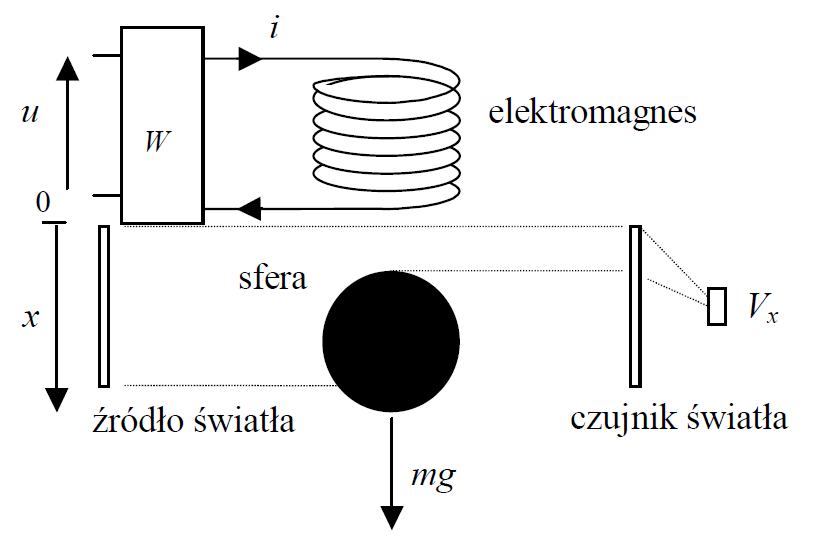
\includegraphics[scale=0.45]{img/model-rownania.PNG}
\caption{Schemat stanowiska służący do wyznaczania równań, źródło \cite{Bania200.}}
\label{rys:model-rownania}
\end{figure}

\begin{equation}\label{modelMagLev}
  \begin{cases}
    \dot x_1 & = x_2 \\
    \dot x_2 & = \dfrac{1}{2m} \dfrac{dL(x_1)}{dx_1} x_3^2(t) + 10^{-3} g  \\
    \dot x_3 & = -\frac{1}{T} x_3(t) + \frac{k}{T} (u(t) + u_c) \\
  \end{cases}  
\end{equation}

Gdzie:
\\$x_{1}$ - położenie sfery $[m]$
\\$x_{2}$ - prędkość sfery $[m/s]$
\\$x_{3}$ - prąd w cewce $[A]$ \newline

\subsection{Analiza modelu}

Zmienne stanu i sterowanie spełniają warunki:
\begin{equation}
\begin{cases}
x_1(t) \in [0, x_{max}] \\
x_2(t) \in R \\
x_3(t) \in [ku_c, k(u_c+u_{max})] \\
u(t) \in [0, u_{max}]
\end{cases}
\end{equation}




\section{Identyfikacja}


\subsection{Identyfikacja charakterystyki czujnika położenia}

Pomiar położenia sfery w układzie magnetycznej lewitacji jest dokonywany optycznie. Z jednej strony znajduje się źródło światła, a po przeciwnej stronie fotodioda z przetwornikiem A/C, która podaje pewne napięcie $u_x$. Podczas identyfikacji poszukujemy zależności tego napięcia od położenia sfery:

\begin{equation} \label{eq:gx}
u_x = g(x_1)
\end{equation}

Poszukujemy charakterystyki statycznej $g(x_1)$, którą otrzymamy przykręcając sferę do śruby i podnosząc ją co ustalony skok 0,7 mm. Za każdym razem dokonujemy pomiaru napięcia podanego przez detektor światła.

Do pracy z modelem potrzebna jest znajomość położenia sfery, dlatego na rysunku \ref{img:gx} charakterystyka odwrotną do zależności \ref{eq:gx}.

\begin{figure}[!htb]
\centering
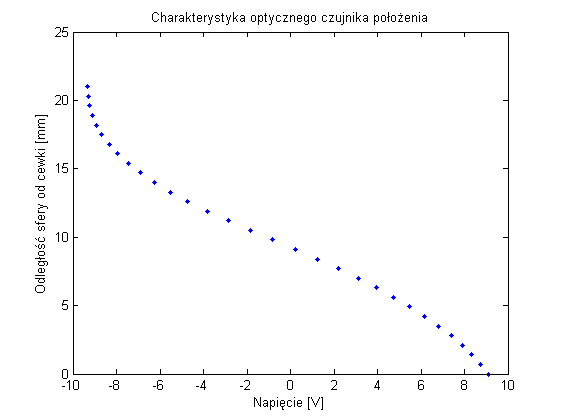
\includegraphics[scale=1]{img/czujnik_polozenia.png}
\caption{Charakterystyka statyczna optycznego czujnika położenia}
\label{img:gx}
\end{figure}


W pracy \cite{Bania1999} autor dokonał aproksymacji otrzymanej charakterystyki odwrotnej sumą funkcji wykładniczych metodą prób i błędów. Nie będziemy dokonywać takiej aproksymacji, ponieważ podczas pracy z modelem w laboratorium użyjemy bloku \textit{LUT z interpolacją} oferowanego przez Simulink.



\subsection{Identyfikacja parametrów cewki $k, T, u_c$ }

Aby wiedzieć, jak zmienia się prąd cewki w zależności od użytego sterowania, czyli przyłożonego napięcia $u$, należy wyznaczyć parametry $k, T$ oraz $u_c$.

\subsubsection{Pomiary w stanie ustalonym cewki}

Zależność prądu od napięcia może być dość dobrze przybliżona funkcją liniową
\begin{equation}
i = k(u + u_c)
\end{equation}

Parametry $k$ i $u_c$ (wzmocnienie oraz stałe napięcie na cewce) wyznaczymy mierząc prąd w stanie ustalonym dla różnych wartości napięcia sterującego. Poniżej przedstawiono wykres obrazujący uśrednione pomiary prądu i przy zadanym sterowaniu. Wyznaczone parametry $k$ i $u_c$ przedstawia tabela \ref{tab:parametry_ident}.


\begin{figure}[!htb]
\centering
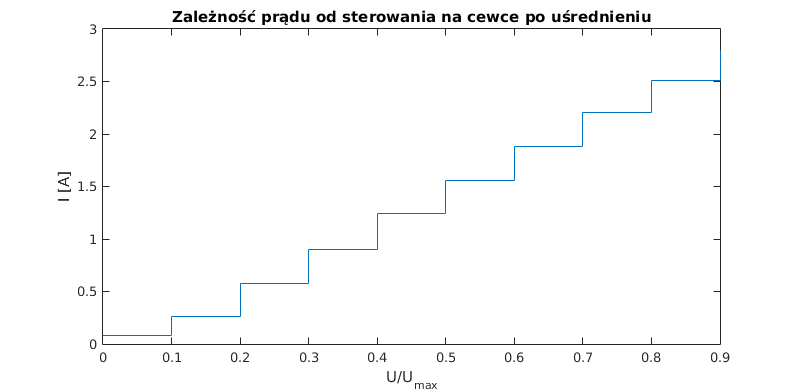
\includegraphics[scale=0.85]{img/prad_cewki_od_sterowania.png}
\caption{Identyfikacja parametrów statycznych cewki}
\label{rys:cewka_k_uc}
\end{figure}

\subsubsection{Pomiary stanów przejściowych cewki}

Stałą czasową cewki $T$ można wyznaczyć obserwując odpowiedź skokową prądu. Aby możliwe było przejście w tryb sterowania pseudo-napięciowego należy zwolnić sygnał sterujący PWM z wypełnieniem 50\%. W tym celu wykorzystano wbudowany preskaler z ustawioną wartością 4096.
\begin{figure}[H]
\centering
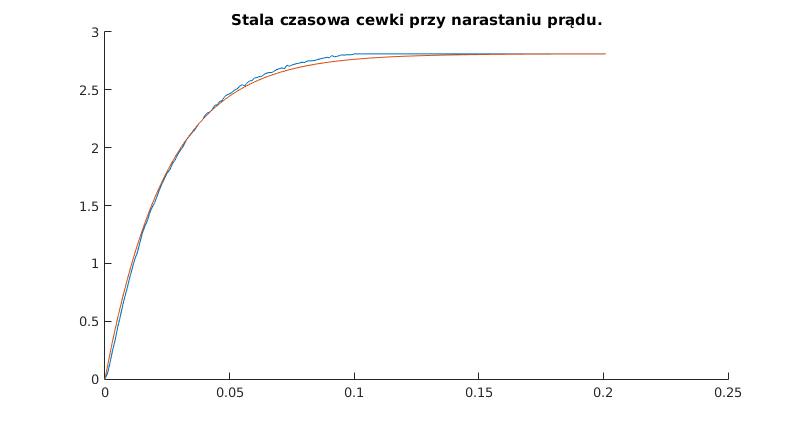
\includegraphics[scale=0.85]{img/identyfikacja_stala_narastanie_0245.png}
\caption{Identyfikacja parametrów statycznych cewki}
\label{rys:cewka_k_uc}
\end{figure}

\begin{figure}[H]
\centering
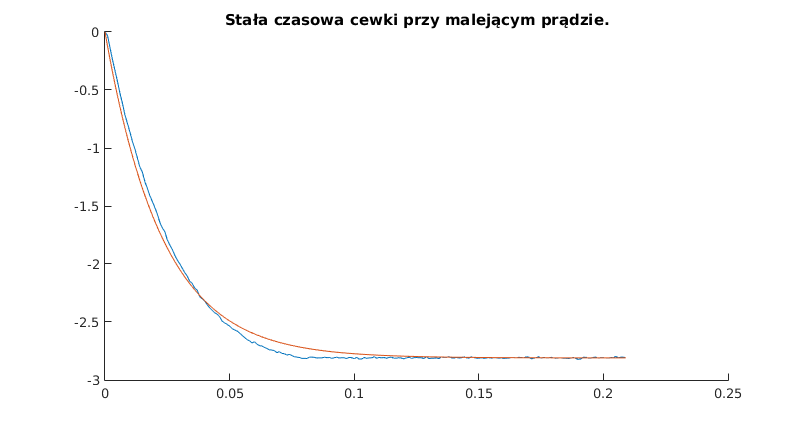
\includegraphics[scale=0.85]{img/identyfikacja_stala_opadanie_0230.png}
\caption{Identyfikacja parametrów statycznych cewki}
\label{rys:cewka_k_uc}
\end{figure}

%\begin{figure}[!ht]
%\centering
%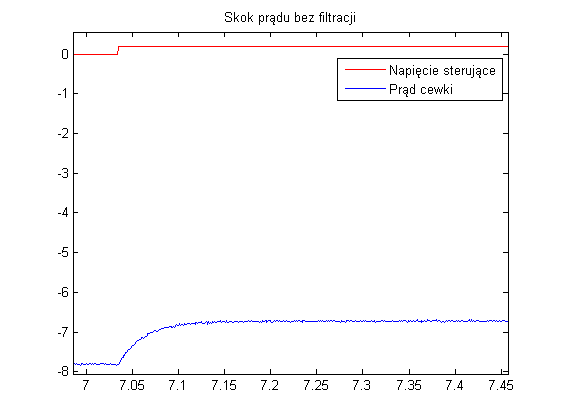
\includegraphics[scale=0.85]{img/skok_pradu_bezfiltra_pwm_szybkie.png}
%\caption{Identyfikacja stałej czasowej narastania prądu cewki [bez filtra, z PWM]}
%\label{rys:skok_pradu_bezfiltra}
%\end{figure}


Korzystając z metody najmniejszych kwadratów wyznaczono parametry, których wartości umieszczono w tabeli  \ref{tab:parametry_ident}.



\subsection{Identyfikacja indukcyjności cewki $L(x_1)$}

W celu identyfikacji zależności indukcyjności cewki od położenia w układzie otwartym należy wykonać serię pomiarów napięcia i prądu dla różnych położeń sfery. Zmierzona rezystancja cewki wynosi $R = 4,7\Omega$. Indukcyjność obliczymy ze wzoru
\begin{equation}
L = \dfrac{1}{\omega}\sqrt{\dfrac{U^2}{I^2} - R^2}
\end{equation}

gdzie
$\omega$ - częstość napięcia zasilającego ($\omega$ = 314 rad/s)

$U$ - napięcie skuteczne na cewce [V]

$I$ - prąd płynący przez cewkę [A]

$R$ - rezystancja cewki


Poszukujemy funkcji postaci
\begin{equation}
L(x_1) = L_0 + 2 \cdot 10^{-3} \dfrac{mg}{a^2x + ab}
\end{equation}
Ze względu na bardzo małe zmiany indukcyjności podczas pomiarów w pętli otwartej, postanowiliśmy użyć regulatora stabilizującego i znaleźć pochodną indukcyjności korzystając z równania drugiego modelu \ref{modelMagLev}.
Z pomocą prowadzącego dobrane zostały nastawy pozwalające uzyskać efekt stabilizacji z wystarczającą dokładnością. Przedstawia je tabela \ref{tab:parametryPID}.

\begin{table}[ht]
\begin{center}
  \begin{tabular}{| l | c | }
    \hline
    człon & wartość \\ \hline
    P 		& 50 \\ \hline
    I 		& 5 \\ \hline
    D 		& 2.5 \\ \hline
    Offset 	& 0.52 \\
    \hline

  \end{tabular}
  \caption{Parametry użytego regulatora PID}
  \label{tab:parametryPID}
\end{center}
\end{table}

Dysponując możliwością ustawiania pozycji sfery mogliśmy przejść do próby wyznaczenia pochodnej indukcyjności. Poszukiwana postać pochodnej funkcji $L$:
\begin{equation} \label{eq:L'}
L'(x) = - 2 \cdot 10^{-3}\dfrac{mg}{(ax + b)^2}
\end{equation}

W stanie ustalonym zachodzi liniowa zależność prądu w stanie ustalonym od położenia:
\begin{equation} \label{eq:Ix}
I(x) = ax + b = k(u + u_c)
\end{equation}

Przypuszczenia te potwierdza rysunek \ref{rys:prad_od_polozenia}, przedstawiający dane zebrane podczas identyfikacji obiektu.

\begin{figure}[H]
\centering
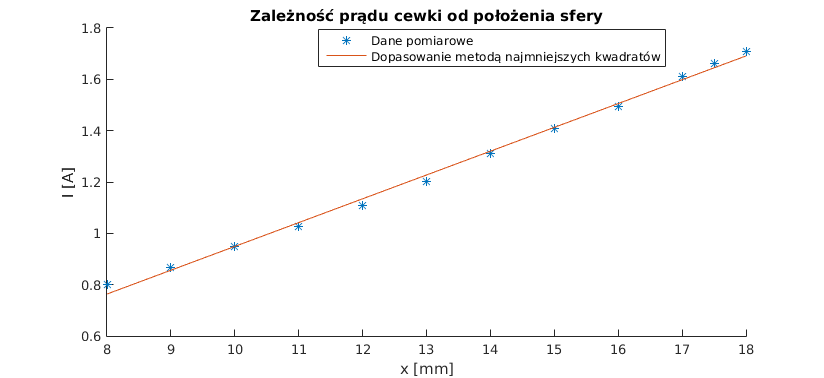
\includegraphics[scale=0.75]{img/identyfikacja_prad_cewki_od_polozenia.png}
\caption{Identyfikacja prądu cewki w funkcji położenia}
\label{rys:prad_od_polozenia}
\end{figure}

Dzięki identyfikacji możliwe było wyznaczenie parametrów prostej wspominanej we wzorze \ref{eq:Ix}, które niezbędne są do wyznaczenia wzoru na pochodną indukcyjności (wzór \ref{eq:L'}).

\begin{figure}[H]
\centering
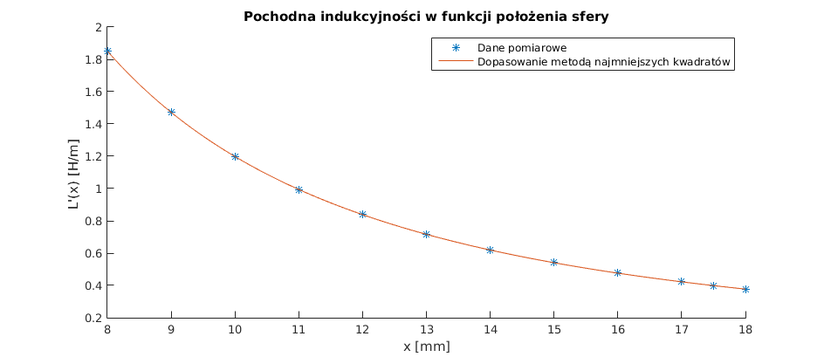
\includegraphics[scale=0.75]{img/identyfikacja_pochodna_indykcyjnosci_od_polozenia.png}
\caption{Identyfikacja pochodnej indukcyjności cewki w funkcji położenia}
\label{rys:pochodna_od_polozenia}
\end{figure}

Wszystkie wyznaczone parametry przedstawia tabela \ref{tab:parametry_ident}.

\begin{table}[H]
\begin{center}
  \begin{tabular}{| l | c | }
    \hline
    parametr 	& wartość \\ \hline
    $k$ & $0.2607$ \\ \hline
    $T_{up}$ & $0.0245 s$  \\ \hline
	$T_{down}$ & $0.023 s$  \\ \hline
	$u_c$ & $-0.0062 $ 	 \\ \hline
    $a$ 		  	& $0.0928$ \\ \hline
    $b$		  	& $0.0214$ \\ \hline
  \end{tabular}
  \caption{Parametry wyznaczone w identyfikacji obiektu}
  \label{tab:parametry_ident}
\end{center}
\end{table}

\subsection{Weryfikacja modelu}

Poniżej przedstawiono porównanie zaproponowanego modelu obiektu wraz ze zidentyfikowanymi parametrami oraz rzeczywistego obiektu. Jak widać rozbieżności są dość spore, jednak w dłuższym horyzoncie czasowym model przyzwoicie oddaje zachowanie się rzeczywistego układu.

\begin{figure}[H]
\centering
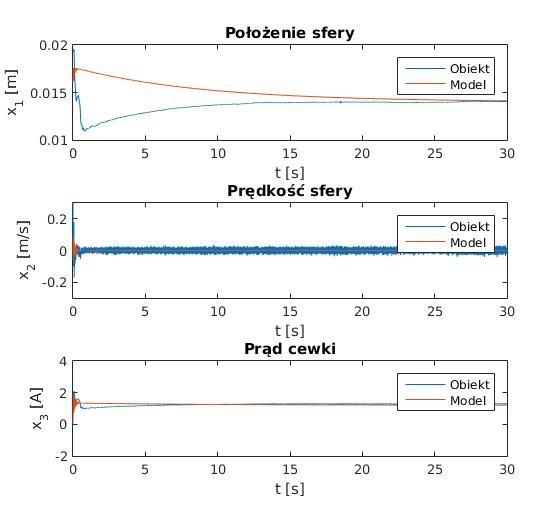
\includegraphics[scale=0.75]{img/zgodnosc_1.png}
\caption{Zachowanie obiektu i modelu - długi horyzont czasowy}
\label{rys:pochodna_od_polozenia}
\end{figure}


\begin{figure}[H]
\centering
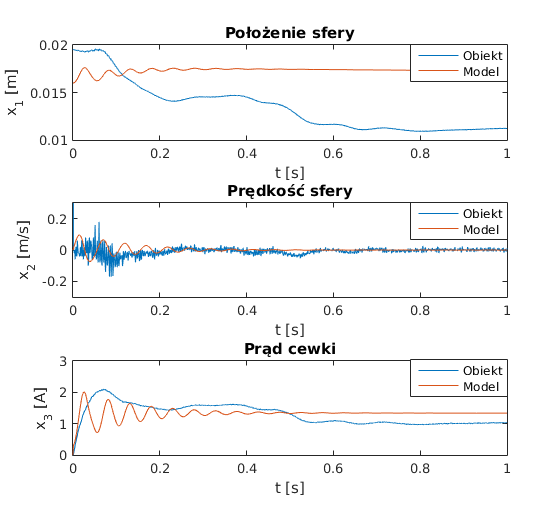
\includegraphics[scale=0.75]{img/zgodnosc_2.png}
\caption{Zachowanie obiektu i modelu - krótki horyzont czasowy}
\label{rys:pochodna_od_polozenia}
\end{figure}

%\begin{figure}[!htb]
%\centering
%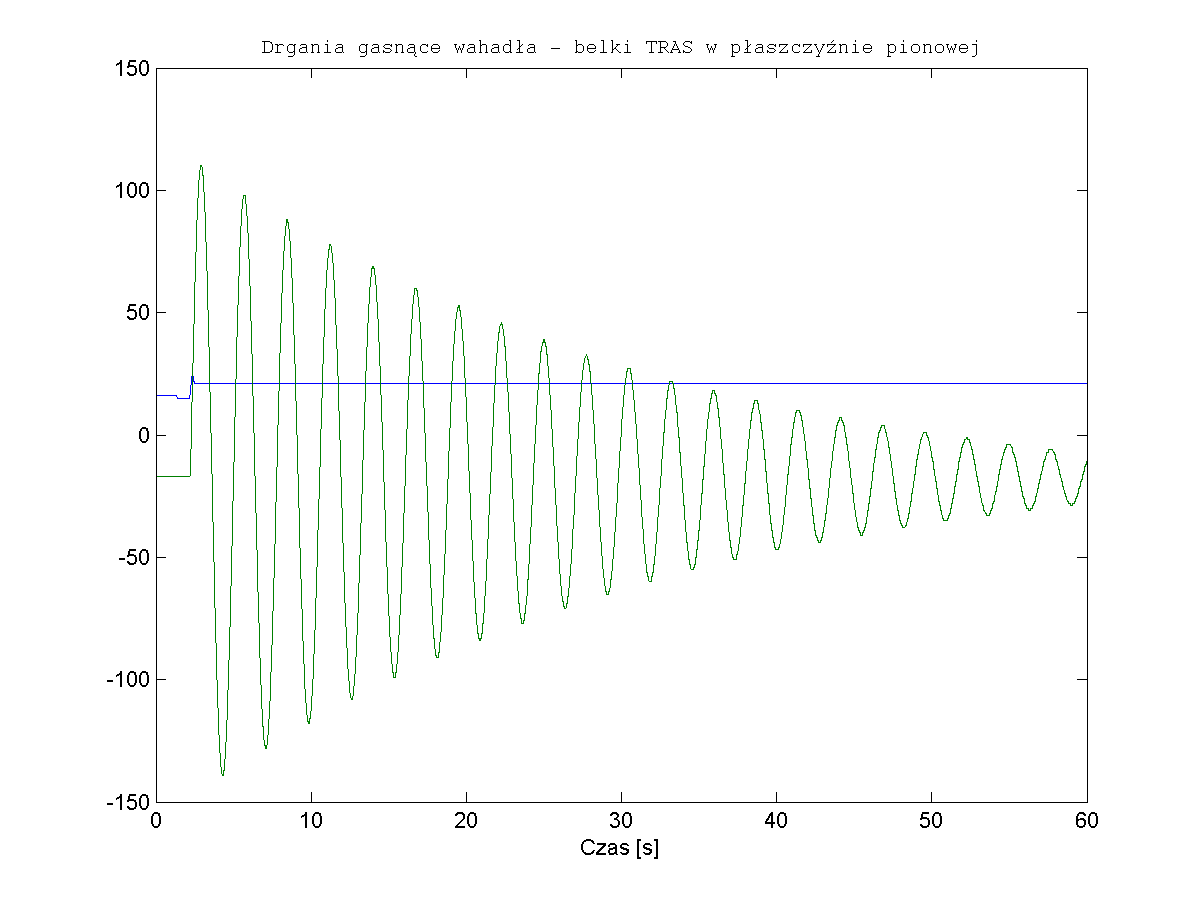
\includegraphics[scale=0.85]{img/gasnace.png}
%\caption{Identyfikacja oporów tarcia belki w płaszczyźnie pionowej}
%\label{rys:gasnace}
%\end{figure}




\bibliography{bib/Bibliografia}
\end{document}